\chapter[Literature Review]{Literature Review}{Literature Review}\label{CH2:LTR}

\section{Introduction}
Low emission combustion techniques such as High Temperature Air Combustion (HiTAC) \cite{CHOI1998,WEBER2020115551,weinberg1971combustion,GuptaHiTAC1999,HiTAC2002,Gupta25280,Gupta1610009,Gupta2436558,LILLE2005373,Mortberg7899,Yang499168}, Flameless Oxidation (FLOX) \cite{wunning2006combustion,WUNNING199781,meier2007flox,COLORADO20102443,LAMMEL4001825}, Moderate and Intense Low Oxygen Dilution (MILD) combustion \cite{CAVALIERE2004329,SZEGO2009429,EFFUGGI302356,EFFUGGI41368,KUMAR20052613,WEBER20052623,DALLY2004418}, Colorless Distributed Combustion (CDC) \cite{VA2011,VAThesis2011,ARGHODE201129,ARGHODE2012822,ARGHODE2013930,ARGHODE20116292,ARGHODE20101631,ARGHODE20111096}, Fuel/Oxidant Direct Injection (FODI) furnace \cite{He2008FlamelessCO,SOBIESIAK199893}, Princeton Asymmetric Whirl Combustor (PAWC) \cite{RHODE60127, YETTER20001265}, High Intensity Low Emission Burner (HILE) \cite{KUMAR20021131}, Jet Stirred Reactor (JSR) \cite{RUTAR20002435} and Trapped Vortex Combustor (TVC) \cite{TVC5266}, Dry Low NOx (DLN) \cite{Vandervort1362661}, Peripheral Vortex Reverse Flow (PVRF) combustor \cite{AHMAD2021100754, AHMAD2023101200,GUPTA2020116766,SOOD2020052302} and Stagnation Point Reverse Flow (SPRF) combustor \cite{bobba2006characteristics,bobba2008SPRF,CJNYJS91338,gopalakrishnan2007effects,DUWIG2014256} is discussed.

\section{High Temperature Air Combustion (HiTAC)}
The novel approach involves heating the reactant air to a significantly high temperature, surpassing that of traditional recuperative combustion. This is achieved by exchanging enthalpy between the furnace section's exhaust gases and the fresh incoming air, facilitating heat and mass transfer \cite{weinberg1971combustion}. Surprisingly, the occurrence of chemical reactions is not dependent on catalysts or reaction promoters in this novel combustion process. The temperature achieved is frequently higher than the fuel-air mixture's auto-ignition temperature, which varies according to the fuel used. This method, known as High Temperature Air Combustion (HiTAC) \cite{WEBER2020115551}, contrasts with conventional preheated air combustion, which primarily aims to increase the flame temperature. HiTAC flames have stable combustion without the need for a flame stabilizer such as a swirler or bluffbody, resulting in a low pressure drop over the combustor \cite{VAThesis2011}.

\begin{wrapfigure}{r}{0.4\textwidth}
    \centering
    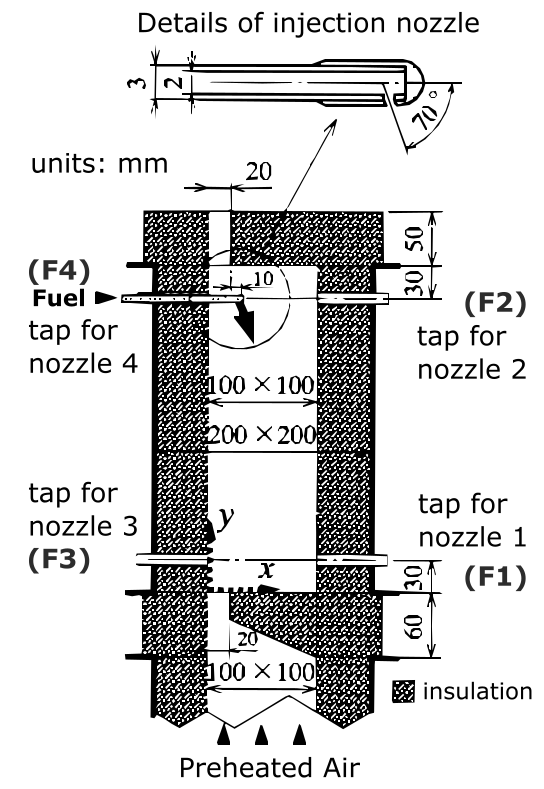
\includegraphics[width=0.4\textwidth]{Chapter2/Images/HiTAC.png}
    \caption[Schematic of HiTAC chamber]{Schematic of HiTAC chamber \cite{CHOI1998}.}
    \label{fig:HiTAC}
\end{wrapfigure}

An investigation was conducted in \cite{CHOI1998} to analyze the impact on fuel mixing conditions by varying fuel injector locations. Preheated air was supplied through a square duct with dimensions of 100 mm $\times$ 100 mm. The combustion chamber had a length of 300 mm and underwent contraction and expansion to create a recirculating flow. The study involved heating air to a temperature of 1423 K using an alternating-flow regenerative preheater. Figure \ref{fig:HiTAC} shows fuel injector locations where CNG was used as fuel. The results showed significant variations in NO (nitric oxide) emissions among the different cases. The lowest NO emissions were observed when fuel was injected at location "F3," which resulted in uniform fuel mixing and suggested distributed combustion. It was found that NO emissions in this case were independent of temperature and equivalence ratio. On the other hand, injecting fuel at location "F2" led to very high NO emissions.

\section{Colorless Distributed Combustion (CDC)}
 \begin{wrapfigure}{r}{0.4\textwidth}
     \centering
     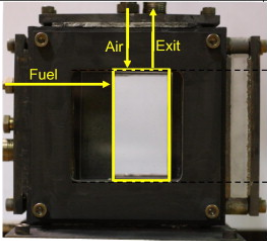
\includegraphics[width=0.37\textwidth]{Chapter2/Images/CDC.png}
     \caption[Experimental setup of CDC]{Experimental setup of CDC \cite{ARGHODE2012822}.}
     \label{fig:CDC}
 \end{wrapfigure}
 
The term "colorless" refers to the flame's low visible emission when compared to conventional flames \cite{ARGHODE201129}. The distributed reaction zone facilitates the distributed combustion, which occurs throughout the entire combustion zone. To achieve reactions similar to those of colorless distributed combustion (CDC), certain conditions must be met. These include separating the air and fuel streams to prevent direct reactions and controlling the product gases entrainment in the air stream to create a high-temperature and low-oxygen oxidizer \cite{ARGHODE201129}. This oxidizer is then mixed with the fuel jet, leading to spontaneous ignition and creating a distributed combustion reaction zone throughout the entire combustion chamber \cite{ARGHODE201129}.

The study conducted in \cite{ARGHODE2013930} investigates CDC and examines the impact of different thermal intensities. The research focuses on thermal intensities ranging from 5 to 453 MW/m3 atm \cite{doi:10.1021/ef402357t}, aiming to achieve improved performance without substantial increase in hardware cost. The study explores various flow field configurations and finds that the reverse cross-flow configuration with increased air injection diameter, shown in Figure \ref{fig:CDC}, is particularly favorable. At a thermal intensity of 53 MW/m3 atm \cite{doi:10.1021/ef402357t}, this configuration achieves low emissions of 4 ppm for NOx and 27 ppm for CO. Further reductions in volume lead to higher thermal intensities and emissions, indicating the potential for significantly increasing thermal intensity while maintaining low emissions.
 
\section{Flameless Oxidation (FLOX)}
In 1997, the term "flameless oxidation" (FLOX) was introduced in \cite{WUNNING199781} to reduce thermal NOx emissions in the furnace by avoiding hot spots. FLOX involves combustion without a visible or audible flame, achieved through internal gas recirculation. It was noted that air preheat with higher temperatures were used in this study, but air preheat is not always necessary for flameless oxidation. Additionally, flameless mode can be achieved by injecting air and fuel in a direct or discrete way as well as in premixed mode.

\begin{figure}[!h]
    \centering    
    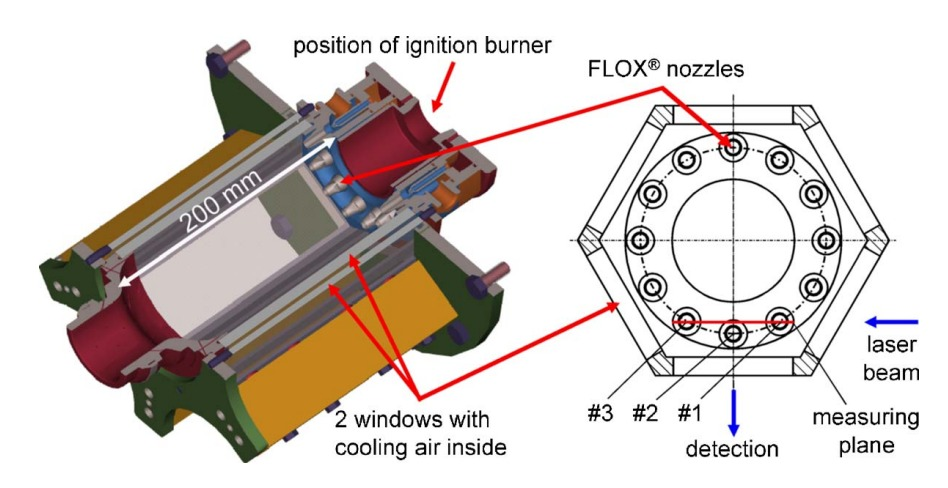
\includegraphics[width=0.7\textwidth]{Chapter2/Images/FLOX.jpeg}
    \caption[FLOX burner]{FLOX burner \cite{LAMMEL4001825}}
    \label{fig:FLOX}
\end{figure}

An enhanced FLOX® burner (see Fig. \ref{fig:FLOX}) was developed and studied in \cite{LAMMEL4001825} to meet the operational requirements of a gas turbine combustor. Compressed natural gas (CNG) and CNG + hydrogen combustion was experimentally and numerically investigated for relevant conditions of gas turbine. Under specific conditions, such as an inlet velocity of 160 m/s and air preheat temperatures of 700 K, low NOx emissions of 10 ppm were achieved with relatively homogeneous flame zones distributed over a large volume. A stable low-emission operating range was achieved for natural gas and high jet exit velocities.  The power densities achieved were 13.3 MW/m3-bar for CNG and 14.8 MW/m3-bar for CNG + H$_2$, meeting the requirements of a gas turbine combustor. The study shows complete and stable combustion with very low pollutant emissions.

\section{Moderate Intense and Low oxygen Dilution (MILD)}

The term "MILD combustion" as discussed in \cite{CAVALIERE2004329} denotes a combustion process distinguished by specific conditions of reactant temperature and temperature increase. In MILD combustion, the reactants' inlet temperature is higher than the mixture's autoignition temperature, however autoignition temperature of the reactant mixture is always higher than temperature increase during the combustion process \cite{doi:10.1021/acs.energyfuels.7b03607}.

\begin{wrapfigure}{r}{0.5\textwidth}
    \centering
    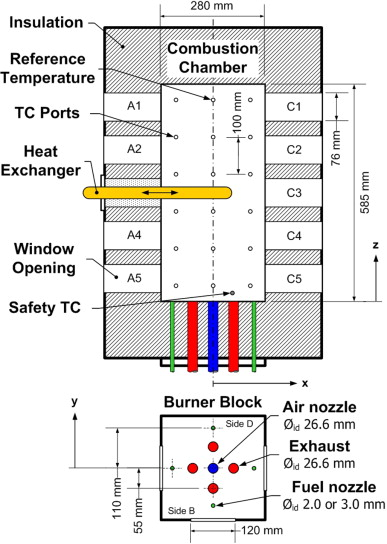
\includegraphics[width=0.5\textwidth]{Chapter2/Images/MILD.jpg}
    \caption[Schematic of MILD combustion]{Schematic of MILD combustion \cite{SZEGO2009429}.}
    \label{fig:MILD}
\end{wrapfigure}

MILD combustion and HiTAC combustion were distinguished based on their respective temperature characteristics. In HiTAC combustion, the temperature rise during the combustion process surpasses reactant's auto-ignition temperature, despite the reactant temperature being higher than the auto-ignition temperature of the reactant mixture \cite{GUPTA2020116766}. This differentiation highlights that in HiTAC combustion, the temperature increase exceeds the threshold for self-ignition, while MILD combustion maintains a temperature rise below the auto-ignition point.

The stability characteristics of MILD combustion burner operating in a reverse flow configuration were investigated in \cite{SZEGO2009429}. The burner had exhaust at centerline of combustion chamber and it is surrounded by four air injection ports at a distance of 55 mm and four fuel injection ports at a distance of 110 mm (see Fig. \ref{fig:MILD}). The study considered various factors such as air preheat temperature, heat extraction, equivalence ratio, and fuel dilution. The baseline case exhibited NOx emissions of approximately 14 ppm. The reduction of the air preheat temperature from 723 K to 300 K led to lower NOx emissions of around 12 ppm. Increasing the amount of heat extraction from 25$\%$ to 42$\%$ led to a significant decrease in NOx emissions, lowering them from 14 ppm to 7 ppm. Surprisingly, as the equivalence ratio increased from 0.8 to 0.9, it resulted in a reduction in NOx emissions from 14 ppm to 8 ppm. Lower NOx emissions were also reported by diluting fuel with CO$_2$ or N$_2$. CO formation is found to be influenced by mixing patterns and furnace temperature rather than heat exchanger effects. The study determines the critical equivalence ratio for low CO emissions, identifies an optimum operating condition, and establishes the significance of fuel jet momentum for system stability. Combustion in MILD regime can be achieved by keeping fuel/air momentum ratio around 0.006 with minimum fuel jet momentum.

\section{Princeton Asymmetric Whirl Combustor (PAWC)}
\begin{wrapfigure}{r}{0.4\textwidth}
    \centering
    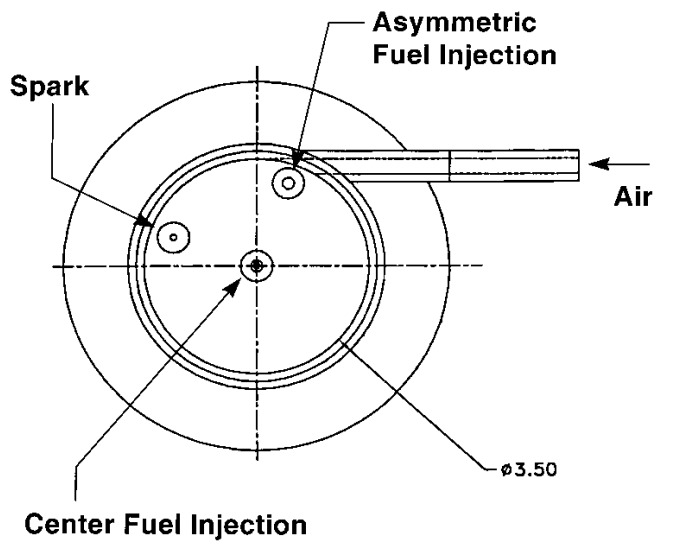
\includegraphics[width=0.4\textwidth]{Chapter2/Images/PAWC.jpeg}
    % \vspace{-2mm}
  \caption[PAWC configuraiton]{PAWC configuraiton \cite{YETTER20001265}.}
  \label{fig:PAWC}
\end{wrapfigure}

A new and promising method for designing low-NOx, non-premixed combustors is introduced in \cite{YETTER20001265}, where fuel is injected in an off-axis or asymmetric manner into a swirling flame. Experimental investigations using this approach were conducted on a laboratory-scale burner, reacting methane and air under atmospheric conditions. The results showed remarkably low NO emissions, measuring below 15 ppm, accompanied by modest CO emissions below 25 ppm at 15$\%$ O$_2$ \cite{YETTER20001265}. The combustor displayed remarkable stability characteristics, even at overall equivalence ratios as low as 0.1 \cite{YETTER20001265}.

\section{Fuel/oxidant direct injection (FODI)}
\begin{wrapfigure}{r}{0.3\textwidth}
\vspace{-10mm}
    \centering
    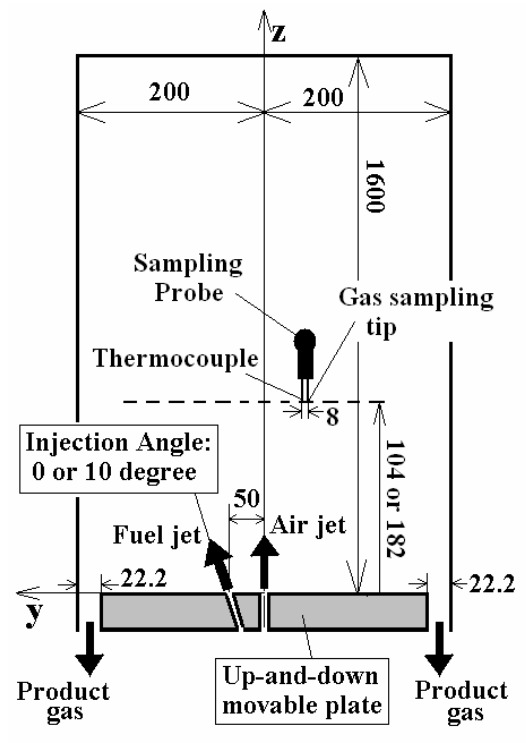
\includegraphics[width=0.3\textwidth]{Chapter2/Images/FODI.jpeg}
  \caption[Schematic of FODI]{Schematic of FODI (units in mm) \cite{He2008FlamelessCO}.}
  \label{fig:FODI}
\end{wrapfigure}

A study on strong-Jet/weak-Jet configuration was conducted in \cite{He2008FlamelessCO}, where air and fuel injected through a single port (see Fig. \ref{fig:FODI}). The air jet with higher momentum was referred to as the ``strong jet", while the fuel jet was called the ``weak jet" \cite{VAThesis2011}. The term ``Fuel/oxidant direct injection (FODI)" was called due to direct injection of air and fuel into the chamber \cite{VAThesis2011}. The combustor operated at 0.1 MW/m3-atm thermal intensity with reverse flow configuration and were able achieve low CO and NOx emissions of 34 ppm and 3 ppm, respectively. The study examined the effects of fuel/air nozzle separation, fuel/air momentum flux, and fuel injection angle in depth \cite{VAThesis2011}. Lower injection angles were found to result in reduced NOx emissions, while higher fuel injection velocities led to greater fuel dilution before combustion, resulting in lower NOx emissions. 

\section{High Intensity Low Emission Burner (HILE)}

\begin{wrapfigure}[13]{r}{0.3\textwidth}
\vspace{-12mm}
    \centering
    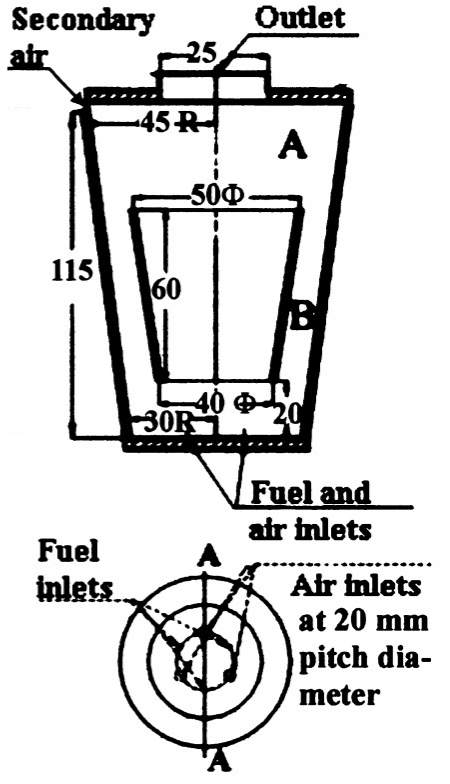
\includegraphics[width=0.3\textwidth]{Chapter2/Images/HILE.png}
    % \vspace{-2mm}
  \caption[Schematic of HILE burner]{Schematic of HILE burner \cite{KUMAR20021131}.}
  \label{fig:HILE}
\end{wrapfigure}

A study conducted on a HILE, combustor specifically designed for high thermal intensity furnace applications in \cite{KUMAR20021131}. Unlike previous studies, which demonstrated thermal intensities below 1 MW/m3-atm, this combustor achieved a thermal intensity of 10 MW/m3-atm. Combustion chamber consists a frustum of cone  (see Fig. \ref{fig:HILE}) to enhance gas recirculation and achieve a notable reduction of 10-15 dB in noise levels. The study showed that to achieve low emissions, high air preheat temperature was not necessary. Recuperator/regenerator system (used in previous studies) was eliminated just by using air and fuel at ambient temperature as peripheral high-speed jets at the bottom. Although low NO$_x$ emissions of approximately 4 ppm were achieved, the combustor exhibited high levels of CO emissions (2300 ppm), even after the use of staged air with a 10$\%$ excess to oxidize CO.

\section{Jet Stirred Reactor (JSR)}

\begin{wrapfigure}{r}{0.4\textwidth}
% \vspace{-20mm}
    \centering
    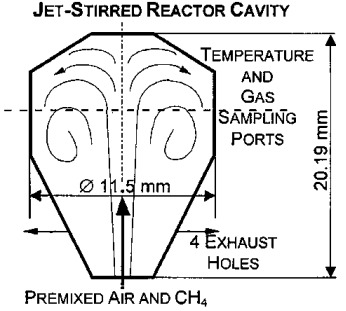
\includegraphics[width=0.33\textwidth]{Chapter2/Images/JSR.jpeg}
    % \vspace{-2mm}
  \caption[Schematic of JSR]{Schematic of JSR \cite{RUTAR20002435}.}
  \label{fig:JSR}
\end{wrapfigure}
A JSR in \cite{RUTAR20002435}, investigated the formation of NOx, operating with lean-premixed methane/air (see Fig. \ref{fig:JSR}). The study analyzed the effects of pressure, residence time, and inlet temperature on NOx formation \cite{RUTAR20002435}. The results showed that lower residence times resulted in lower NOx levels, while higher concentrations were observed at extreme residence times. Increasing pressure and inlet temperature had a reducing effect on NOx concentrations. Concentration profiles within the reactor indicated two distinct regions: a postflame region and a highly CO concentrated non-equilibrium reaction zone. NOx formation mainly occurred in the non-equilibrium reaction zone. The study also identified a chemical rate-limiting  and high-intensity combustion regimes based on the Damköhler number and the ratio of turbulent intensity to laminar burning velocity \cite{RUTAR20002435}.

\section{Trapped Vortex Combustor (TVC)}

\begin{wrapfigure}{r}{0.4\textwidth}
% \vspace{-8mm}
    \centering    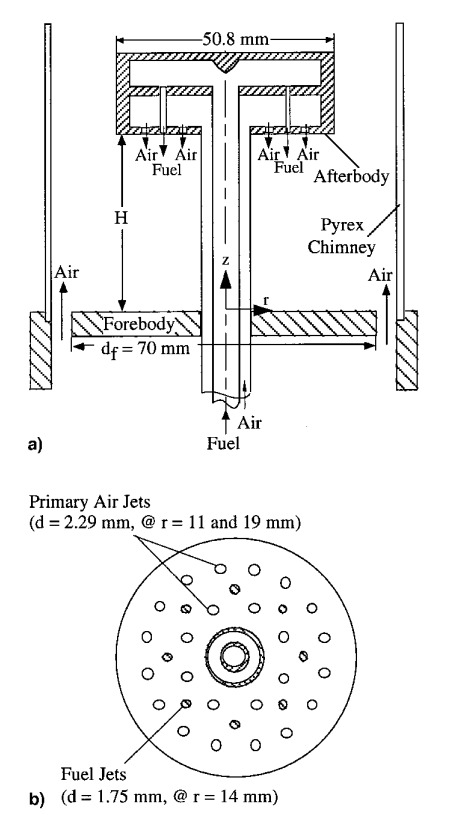
\includegraphics[width=0.4\textwidth]{Chapter2/Images/TVC.jpeg}
    \caption[Schematic of TVC]{Schematic of TVC \cite{TVC5266}.}
    \label{fig:TVC}
\end{wrapfigure}

TVC technology in \cite{TVC5266} utilizes a unique approach to enhance flame stability by injecting fuel into a confined vortex located between two plates or within a cavity along the combustion airflow path (see Fig. \ref{fig:TVC}). This design enables the formation of a concentrated burning reaction zone within the small cavity, resulting in exceptional lean operational limits with an overall equivalence ratio below 0.2. 
The trapped vortex acts as a continuous ignition source for combustion, as the mixture within it is typically rich \cite{RUTAR20002435}, generating highly reactive hot gases that readily ignite the mixture in the main combustion chamber.
The TVC exhibits a low lean blowout (LBO) limit across a broad operating range due to the shielding of the cavity from the annular air. Without primary air, the length of the cavity strongly influences the LBO limit, with an optimal length of 0.6 times the diameter of the Forebody. Residence time and mixing directly affects the LBO limit in the presence of primary air.
Lower LBO limits are achieved at lower primary air flow rates, while higher primary air flows result in a linear increase in the fuel flow rate at the LBO limit. Additionally, the TV-combustor demonstrates a low-pressure drop, offering potential reductions in specific fuel consumption. At a low annular air velocity of 14 m/s, combustion efficiencies were around 99$\%$, decreasing to 97$\%$ at a higher velocity of 42 m/s, and reaching 99$\%$ with the inclusion of a second cavity. At higher annular air flows, combustion showed a narrower high-efficiency range due to its sensitivity to the primary air. The primary zone is believed to be the primary source of NOx formation.

\newpage
\section{Dry Low NOx (DLN)}
\vspace{-5mm}
\begin{wrapfigure}[12]{r}{0.3\textwidth}
\vspace{-12mm}
    \centering    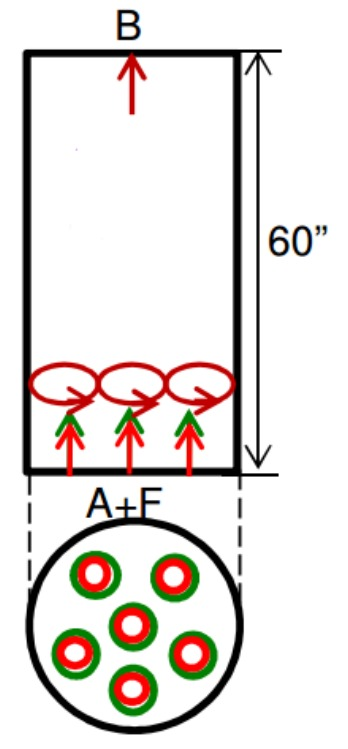
\includegraphics[width=0.25\textwidth]{Chapter2/Images/DLN.jpeg}
    \caption[DLN combustor]{DLN combustor \cite{SKG2017}.}
    \label{fig:DLN}
\end{wrapfigure}

The core principle of this combustor is to generate a well-mixed combination of lean air and fuel prior to its introduction into the combustion chamber of a gas turbine. Flame temperature remains relatively low by maintaining lean mixture, resulting in decreased NOx emissions \cite{SKG2017}. 

A DLN combustor investigated in \cite{Vandervort1362661} operates at 15MW/m3-atm thermal intensity and a length scale of 1.52 m (see Fig. \ref{fig:DLN}). It achieves low emissions, with NOx and CO levels below 9 ppm for load conditions ranging from 50$\%$ to 100$\%$. Operating at an inlet temperature of 631K, outlet temperature of 1561K, and an operating pressure of 16 atm, it is applied in GE-7FA gas turbine combustors. The DLN combustion method utilizes lean premixed combustion and fuel staging to effectively reduce NOx emissions across various load conditions.

\section{Peripheral Vortex Reverse Flow (PVRF)}

\begin{wrapfigure}{r}{0.35\textwidth}
\vspace{-5mm}
    \centering
    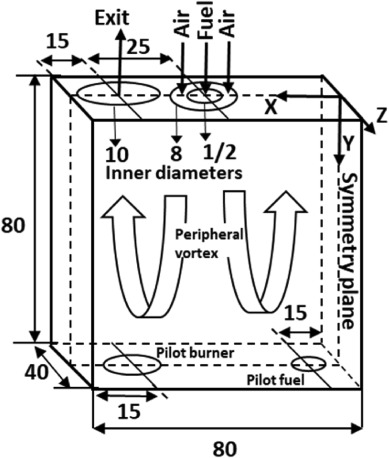
\includegraphics[width=0.35\textwidth]{Chapter2/Images/PVRF.jpg}
    \caption[Schematic of PVRF combustor]{Schematic of PVRF combustor \cite{AHMAD2023101200}.}
    \label{fig:Ch2PVRF}
\end{wrapfigure}

PVRF combustor operates using a reverse flow design. In this combustor, air injects along the center line of the combustor and when the air jet reaches the bottom of the combustor, it splits into two streams, creating two recirculation zones on either side of the air jet due to the reversal of flow \cite{AHMAD2021100754}. The recirculation zone located near the sidewall and away from the combustor exit in figure \ref{fig:Ch2PVRF} is referred to as the ``peripheral vortex'' \cite{AHMAD2021100754}. This peripheral vortex plays a crucial role in entraining the hot product gases and contributing to the stabilization of reactions.

The PVRF combustor in \cite{AHMAD2023101200} is examined with a maximum 6.25 kW heat load and 25 MW/m3-atm thermal intensity using ethylene and LPG fuels in both non-premixed and premixed case. Different fuel injection diameters are tested. In the premixed case, maximum NOx emissions of up to 15 ppm and 26 ppm were observed for LPG and ethylene fuels, respectively, at an equivalence ratio of 0.8. Surprisingly, premixed mode reported higher NOx emissions (for both fuels) than non-premixed case. When using LPG fuel, CO emissions were around 100 ppm and 200 ppm for non-premixed premixed case, respectively. However, with ethylene fuel, the premixed case showed higher CO emissions than the non-premixed case.

\section{Stagnation Point Reverse Flow (SPRF)}

SPRF is a type of low-emission combustor that features a reverse flow configuration. In this technique, along the center line of the combustor, the reactants are injected coaxially. Upon injection, the reactant jet impinges on the combustor's bottom wall, creating a stagnation zone. This zone splits the reactant jet into two symmetrical streams, resulting in a high turbulence and low velocity region known as the ``stagnation point" \cite{bobba2008SPRF}. Additionally, the combustor design promotes internal recirculation of the hot product gases due to the reverse flow configuration. This unique geometry contributes to the low emissions characteristic of the SPRF combustor.

\begin{figure}[!ht]
    \centering
    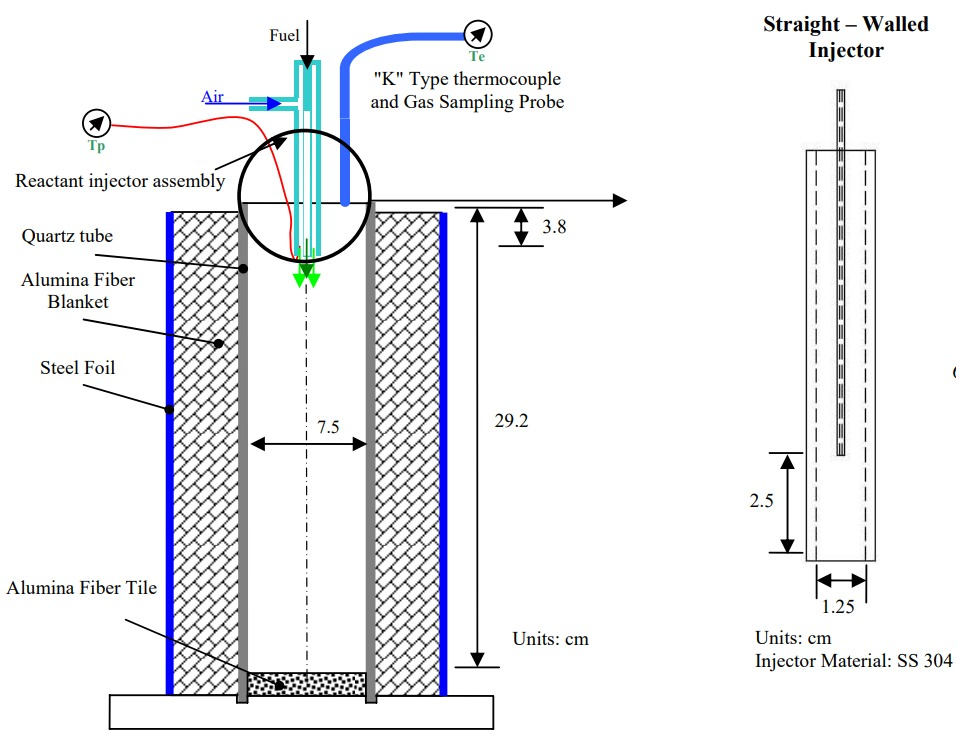
\includegraphics[width=0.8\textwidth]{Chapter2/Images/SPRF_.jpeg}
    \caption[Experimental setup of SPRF combustor]{Experimental setup of SPRF combustor \cite{CJNYJS91338}.}
    \label{fig:Ch2SPRF}
\end{figure}

SPRF combustor investigated in \cite{CJNYJS91338} using an airblast fuel injector to assess the performance of the combustor using Jet-A and heptane liquid fuels. This air blaster was designed for lower mass flux during experiments (see Fig. \ref{fig:Ch2SPRF}). Pressure lossess were kept below 5$\%$ using a diffuser. Jet-A fuel showed a stable combustion at heat intensity of 10 MW/m3-atm. Lower NOx emissions (below 1 ppm) and CO emissions (5 ppm) were reported \cite{10.1115/1.4043437}.

\section{Objectives}
The current thesis deals with the numerical and experimental investigation of a reverse flow configuration for PVRF and SPRF combustor with the following objectives:
\begin{enumerate}
    \item To simulate flow field, temperature field characterstics and gas recirculation of air/fuel mixing. 
    \item To measure the pollutant emissions for a range of equivalence ratios.
    \item To investigate reaction zone positioning using CH* chemiluminescence imaging and direct flame photography.
    \item Compare the results for both PVRF and SPRF combustor.
\end{enumerate}
